\section{Descriptive Statistic}

\subsection{Summary Statistics}
\begin{figure}[H]
    \begin{center}
    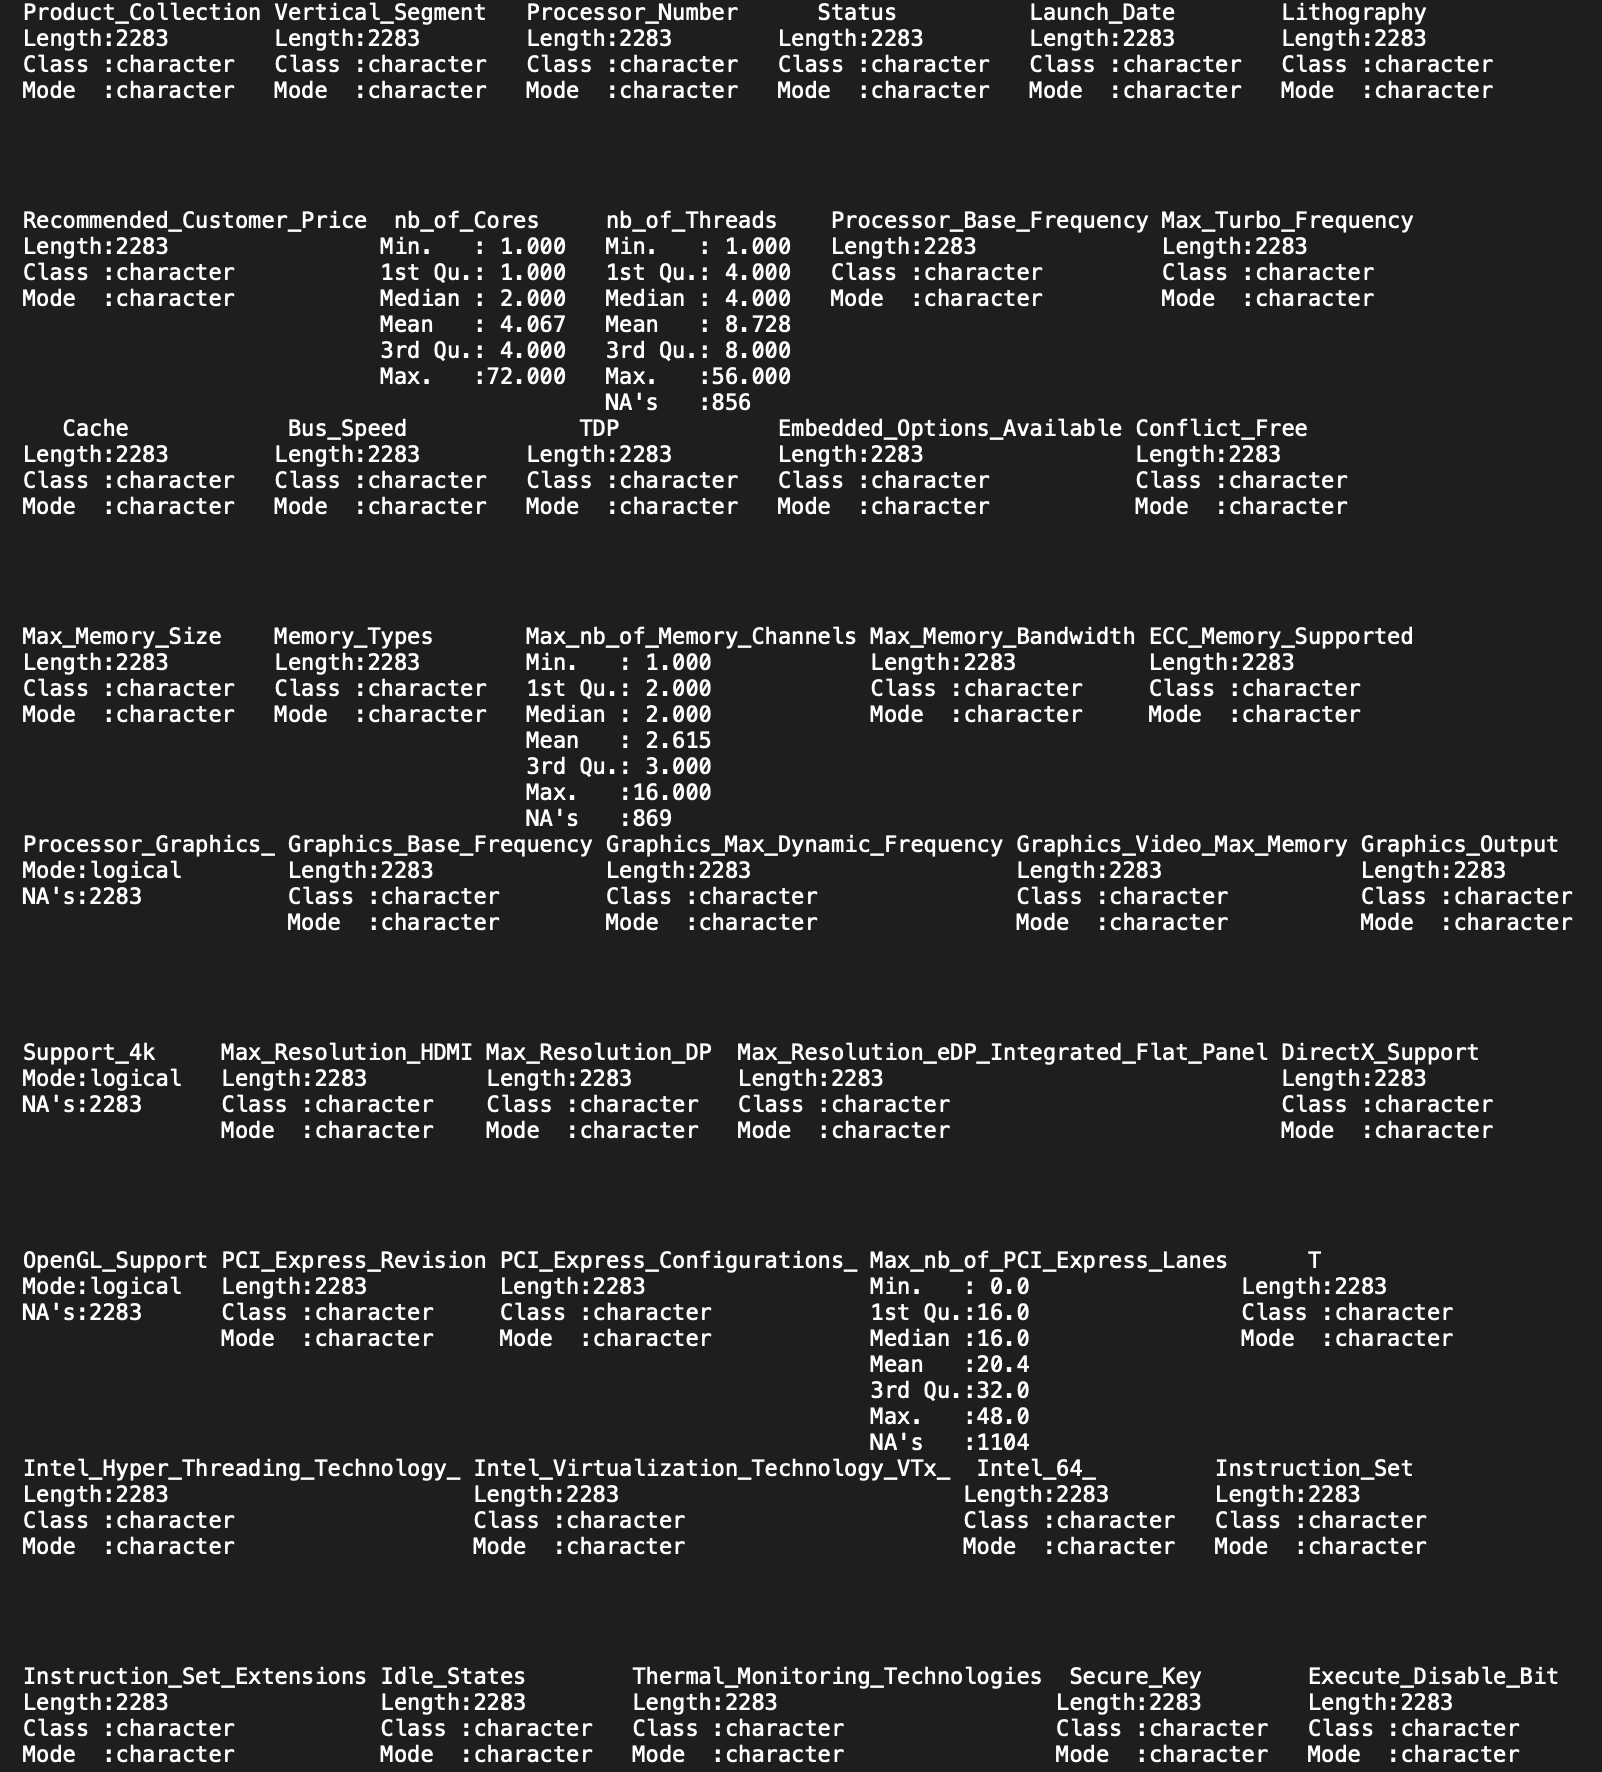
\includegraphics[width=14cm]{graphics/summary.png}
    \end{center}
\end{figure}

\subsection{Distribution and Histograms}
\begin{figure}[H]
    \begin{center}
    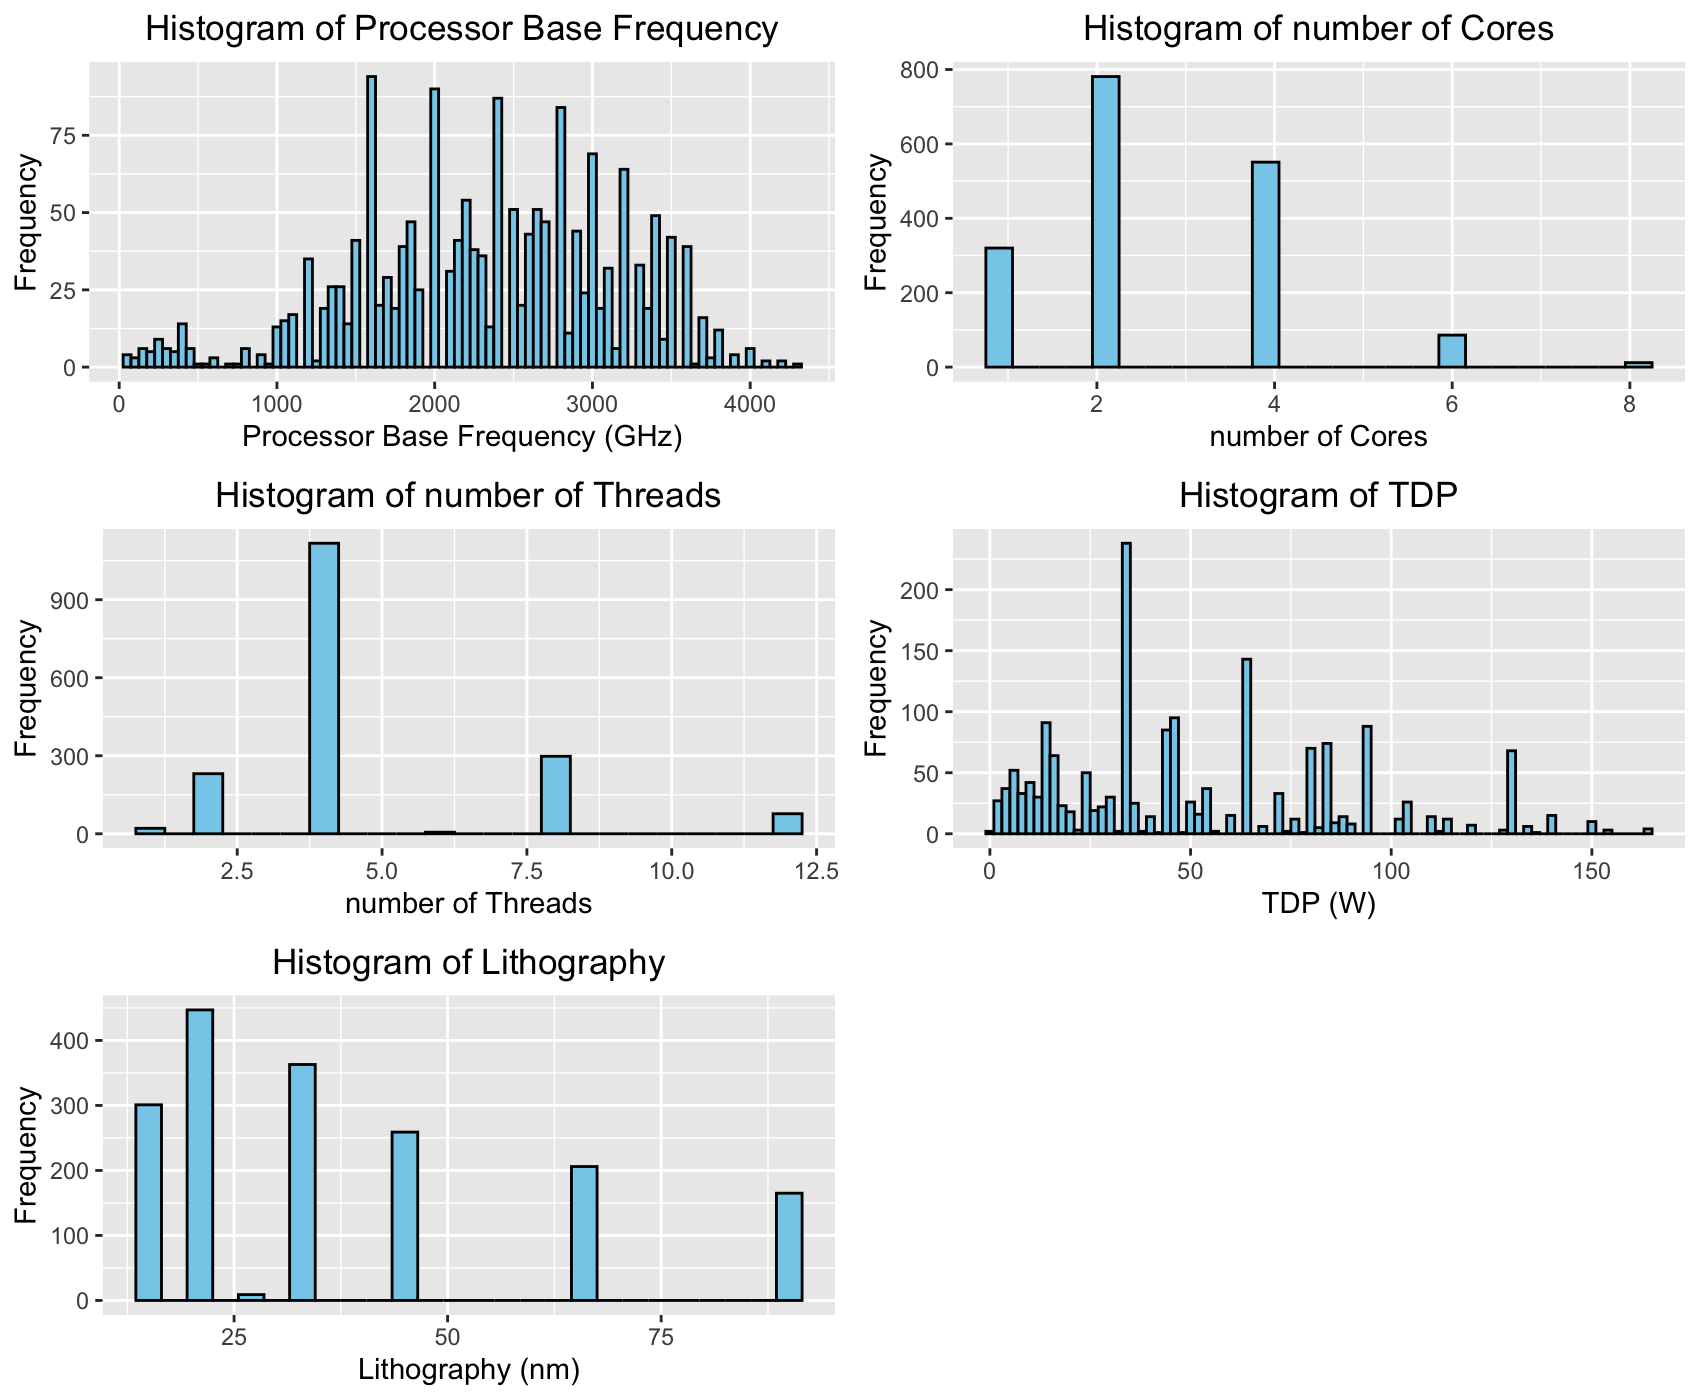
\includegraphics[width=14cm]{graphics/histogram.png}
    \end{center}
\end{figure}
\begin{itemize}
    \item Processor Base Frequency: 
    \begin{itemize}
        \item The distribution of processor base frequencies is relatively normal, with most CPUs having base frequencies between 2 and 3 GHz.
        \item A few CPUs have base frequencies below 2 GHz and above 3 GHz, indicating that while the majority of CPUs fall within a mid-range frequency, there are some outliers at both ends.
    \end{itemize}
    
    \item Number of Cores: 
    \begin{itemize}
        \item The distribution of the number of cores is right-skewed, with a large number of CPUs having between 2 and 8 cores.
        \item There are fewer CPUs with higher core counts, and very few CPUs exceed 16 cores.
        \item This suggests that while multi-core processors are common, high-core-count CPUs are less frequent.        
    \end{itemize}

    \item Number of Threads: 
    \begin{itemize}
        \item Similar to the number of cores, the distribution of the number of threads is right-skewed.
        The majority of CPUs have between 2 and 16 threads.
        \item There are some CPUs with a significantly higher number of threads, indicating the presence of high-performance CPUs with technologies like Hyper-Threading.     
    \end{itemize}

    \item TDP (Thermal Design Power):
    \begin{itemize}
        \item The distribution of Thermal Design Power (TDP) shows that most CPUs have a TDP between 50 and 125 watts.
        \item There are a few CPUs with higher TDP values, which typically correspond to more powerful processors that require more cooling.
        \item This indicates that most CPUs are designed to operate within a standard thermal envelope, but high-performance CPUs demand more power.
    \end{itemize}

    \item Lithography: 
    \begin{itemize}
        \item The lithography histogram shows several peaks, indicating different manufacturing process nodes.
        \item The most common process nodes are 14 nm and 22 nm.
        \item There are also CPUs manufactured at smaller nodes like 10 nm, and larger nodes like 32 nm and 45 nm.
        \item This reflects the advancements in semiconductor manufacturing technology, with newer CPUs being produced at smaller process nodes for improved performance and efficiency.
    \end{itemize}

\end{itemize}

Implications:
\begin{itemize}
    \item Processor Base Frequency: The relatively normal distribution suggests a common range of base frequencies, with few extreme values. This will influence our regression model, as we need to account for these outliers.

    \item Number of Cores and Threads: The right-skewed distributions indicate that while multi-core and multi-threading capabilities are common, the extent varies widely. High-core and high-thread CPUs, although fewer, represent the high-performance segment and should be carefully considered in our model.

    \item TDP: The distribution suggests that most CPUs are designed within certain power and thermal limits, but there are high-performance CPUs with higher TDP. This attribute is crucial as it impacts the CPU's ability to sustain higher clock speeds under load.

    \item Lithography: The presence of multiple peaks reflects the evolution of manufacturing processes over time. This attribute is essential for our model as newer process nodes typically allow for higher clock speeds and better efficiency.
\end{itemize}
By understanding these distributions, we can better prepare our data for inferential statistics and modeling, ensuring that our regression model accurately captures the relationship between these attributes and CPU clock speeds. This will involve handling outliers appropriately, scaling the features, and ensuring that the model is trained on a representative sample of the data.

\subsection{Boxplots for Outliers}
\begin{figure}[H]
    \begin{center}
    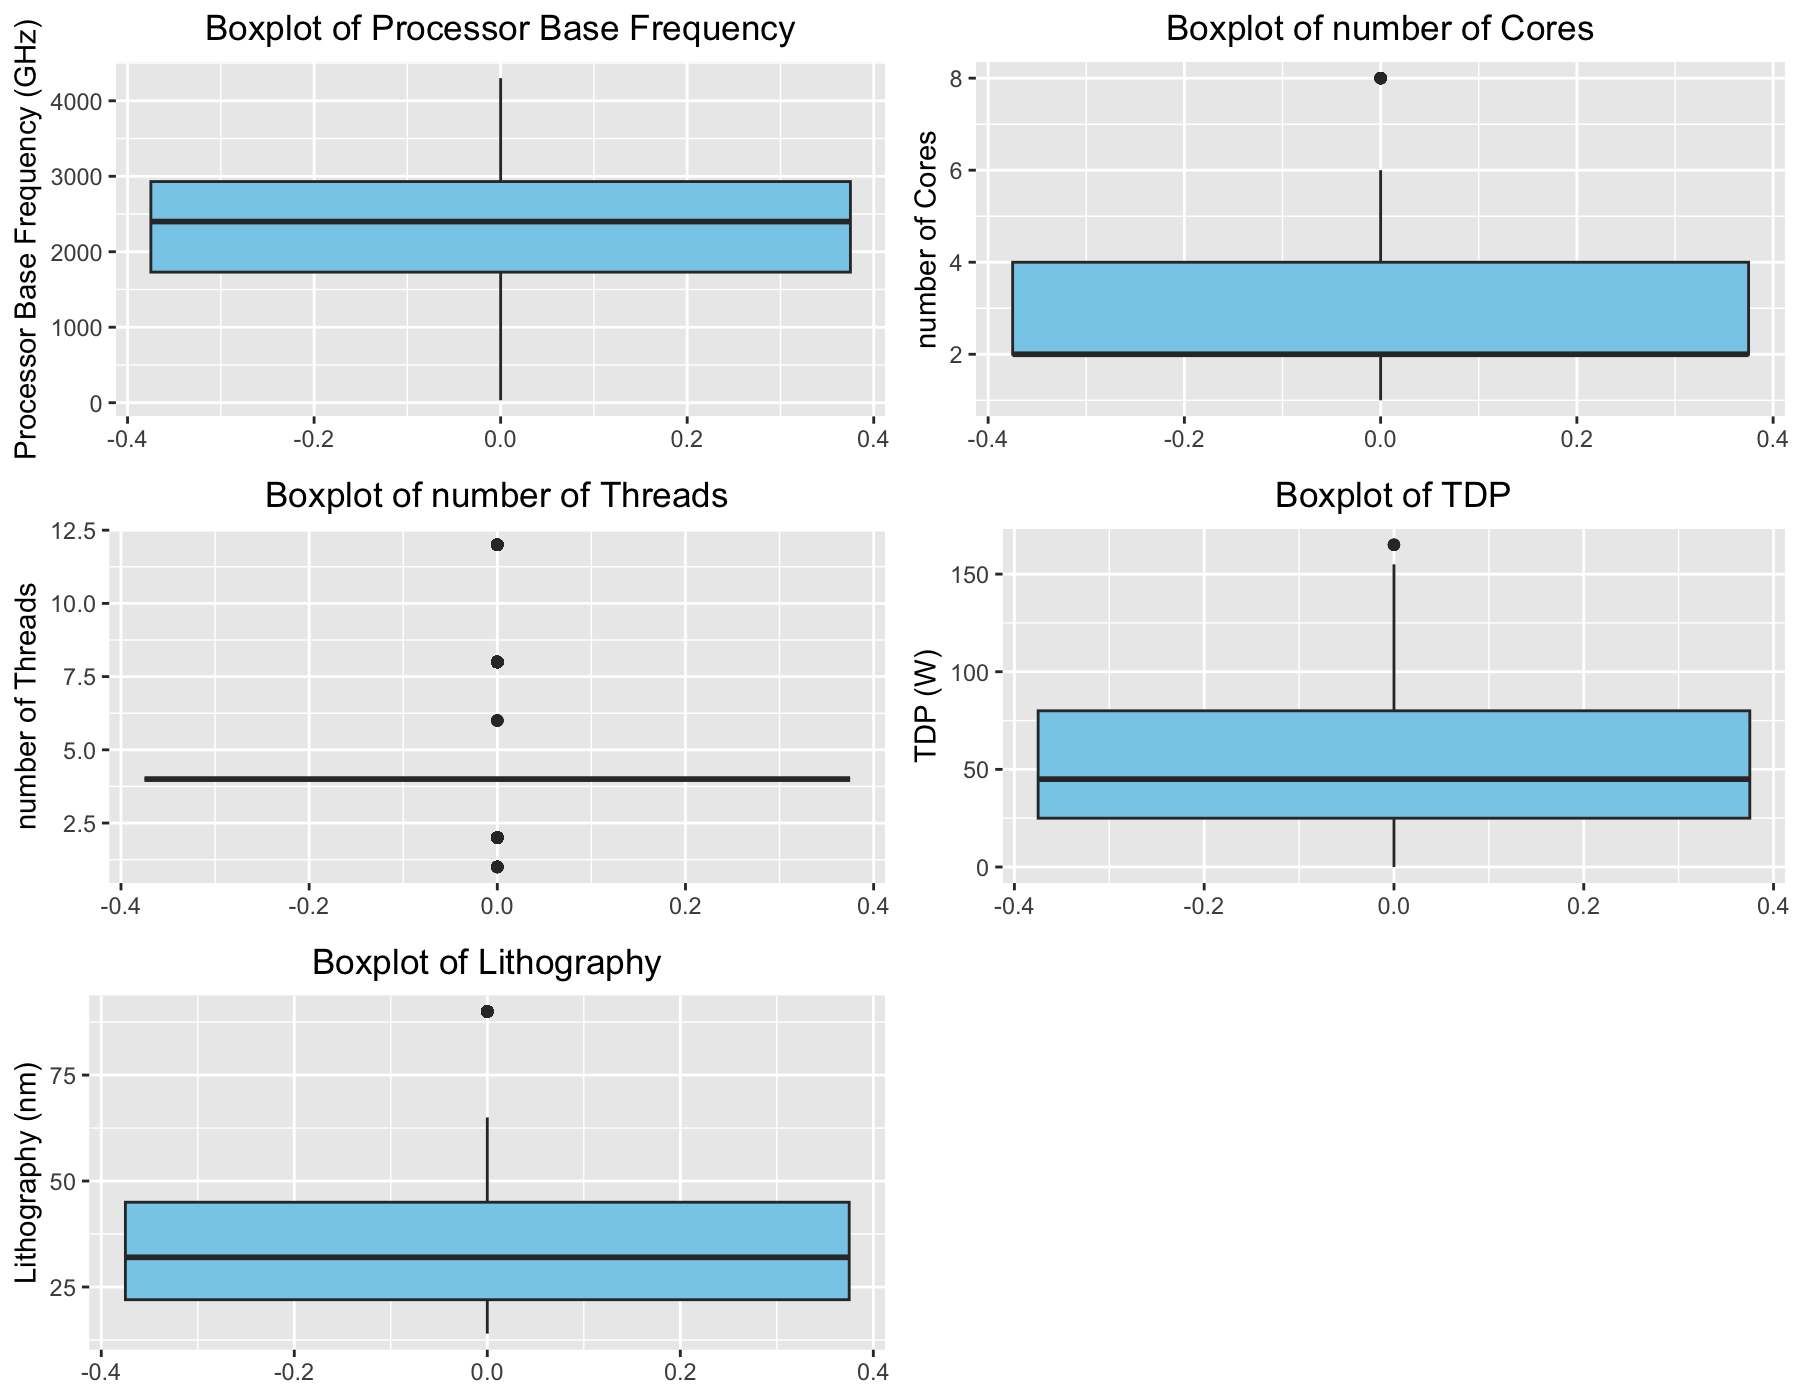
\includegraphics[width=14cm]{graphics/boxplot.png}
    \end{center}
\end{figure}
The boxplots provide a visual representation of the distribution, central tendency, and variability of key attributes in the dataset, as well as the presence of outliers. Here's a detailed explanation of each boxplot:

\begin{itemize}
    \item Boxplot of Processor Base Frequency (GHz):
    \begin{itemize}
        \item The boxplot shows the median processor base frequency around 2.5 GHz, with the interquartile range (IQR) spanning from approximately 2 GHz to 3 GHz.
        There are a few outliers above 3.5 GHz, indicating that some CPUs have significantly higher base frequencies than the majority.
    \end{itemize}

    \item Boxplot of Number of Cores:
    \begin{itemize}
        \item The median number of cores is around 4, with the IQR ranging from 2 to 6 cores.
        \item Numerous outliers are present above 8 cores, reflecting that high-core-count CPUs, while less common, are still significant.
    \end{itemize}

    \item Boxplot of Number of Threads:
    \begin{itemize}
        \item The median number of threads is around 4, with an IQR from 4 to 8 threads.
        \item There are many outliers above 16 threads, indicating that some CPUs, likely with Hyper-Threading, support a significantly higher number of threads.
    \end{itemize}
    
    \item Boxplot of TDP (W):
    \begin{itemize}
        \item The median TDP is around 65 W, with the IQR ranging from approximately 55 W to 95 W.
        \item There are several outliers below 50 W and above 125 W, showing that while most CPUs fall within a certain thermal range, some require much less or much more cooling capacity.
    \end{itemize}

    \item Boxplot of Lithography (nm):
    \begin{itemize}
        \item The median lithography value is 22 nm, with the IQR ranging from 14 nm to 32 nm.
        \item There is one outlier at 65 nm, indicating an older manufacturing process compared to the more advanced and common nodes.
    \end{itemize}
\end{itemize}

Implications:
The boxplots provide several insights that are crucial for our project on predicting CPU clock speeds:

\begin{itemize}
    \item Processor Base Frequency:
    \begin{itemize}
        \item The central tendency and spread of base frequencies are important for understanding the typical performance range of CPUs in the dataset.
        \item The presence of outliers indicates that while most CPUs have base frequencies in a common range, some high-performance CPUs exist with higher base frequencies, which need to be considered in our model.
    \end{itemize}
    
    \item Number of Cores and Threads:
    \begin{itemize}
        \item The distributions show that multi-core and multi-threaded CPUs are common, but high-core and high-thread counts are less frequent, representing high-performance segments.
        \item Outliers in these attributes reflect high-performance CPUs, which can affect the overall performance trends and must be accurately modeled.
    \end{itemize}
    
    \item TDP:
    \begin{itemize}
        \item The central tendency and variability in TDP indicate the power and thermal characteristics of most CPUs.
        \item The outliers suggest that while most CPUs operate within a standard thermal range, some require much higher or lower power, influencing their ability to sustain higher clock speeds.
    \end{itemize}
    
    \item Lithography:
    \begin{itemize}
        \item The distribution of lithography values highlights the evolution of manufacturing technology, with most CPUs produced using advanced nodes like 14 nm and 22 nm.
        \item The outlier at 65 nm represents older technology, which typically correlates with lower efficiency and performance.
    \end{itemize}
\end{itemize}

\subsection{Correlation Matrix}
\begin{figure}[H]
    \begin{center}
    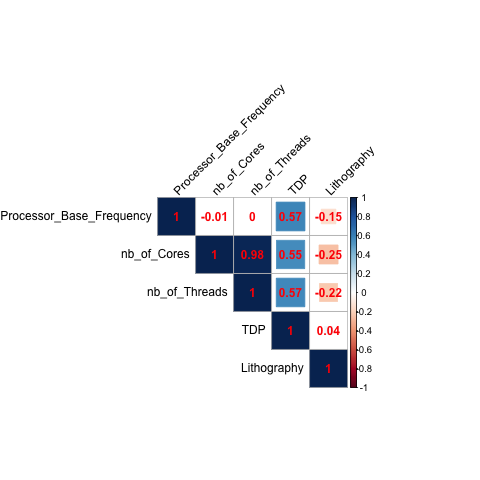
\includegraphics[width=14cm]{graphics/corr_matrix.png}
    \end{center}
\end{figure}

The correlation matrix provides a comprehensive view of the linear relationships between pairs of variables in our dataset. Each cell in the matrix represents the correlation coefficient between two variables, ranging from -1 (perfect negative correlation) to 1 (perfect positive correlation). Here's a detailed explanation of the matrix for our project:\\[6pt]
Key Observations:
\begin{itemize}
    \item Processor Base Frequency:
    \begin{itemize}
        \item Correlation with TDP: The strongest positive correlation is with TDP (0.57). This indicates that CPUs with higher base frequencies generally have higher thermal design power requirements. This is expected as higher clock speeds typically result in greater power consumption and heat generation.
        \item Negative Correlation with Lithography: There is a moderate negative correlation with Lithography (-0.15). This suggests that CPUs manufactured with smaller process nodes tend to have higher base frequencies. Advanced manufacturing technologies often result in better performance characteristics.
    \end{itemize}
    
    \item Number of Cores:
    \begin{itemize}
        \item Strong Positive Correlation with Number of Threads (0.98): This high correlation is expected as CPUs with more cores generally support more threads, especially with technologies like Hyper-Threading.
        \item Negative Correlation with Lithography (-0.25): Indicates that CPUs with a higher number of cores tend to be manufactured using smaller lithography nodes, aligning with advancements in CPU design that pack more cores into smaller spaces.
    \end{itemize}
    
    \item Number of Threads:
    \begin{itemize}
        \item Positive Correlation with TDP (0.57): Similar to the base frequency, a higher number of threads is associated with higher TDP, reflecting increased power consumption and heat dissipation needs.
    \end{itemize}
    
    \item TDP:
    \begin{itemize}
        \item Slight Positive Correlation with Lithography (0.04): This weak correlation suggests that the thermal design power does not have a strong relationship with the manufacturing process node.
    \end{itemize}
    
    \item Lithography:
    \begin{itemize}
        \item Negative Correlations with Other Variables: Lithography shows a general negative correlation with performance-related attributes, reinforcing the trend that smaller manufacturing nodes (indicative of newer technologies) are associated with higher performance capabilities.
    \end{itemize}
\end{itemize}

Implications:
\begin{itemize}
    \item The correlation matrix is crucial for understanding the relationships between different CPU attributes and their collective impact on clock speed. Here are some key takeaways for our project on predicting CPU clock speeds:
    
    \item TDP and Processor Base Frequency: The strong positive correlation suggests that models predicting clock speed should account for TDP as a significant predictor.
    
    \item Manufacturing Process (Lithography): The negative correlations with performance attributes highlight the importance of considering lithography advancements in performance modeling.
    
    \item Number of Cores and Threads: The strong inter-correlation indicates that either variable could be used interchangeably in some modeling contexts, but including both provides a more nuanced understanding of CPU capabilities.
\end{itemize}


\newpage